\documentclass{sigchi-ext}
% Please be sure that you have the dependencies (i.e., additional
% LaTeX packages) to compile this example.
\usepackage[T1]{fontenc}
\usepackage{textcomp}
\usepackage[scaled=.92]{helvet} % for proper fonts
\usepackage{graphicx} % for EPS use the graphics package instead
\usepackage{balance}  % for useful for balancing the last columns
\usepackage{booktabs} % for pretty table rules
\usepackage{ccicons}  % for Creative Commons citation icons
\usepackage{ragged2e} % for tighter hyphenation

\usepackage{marginnote}
%\usepackage{etoolbox}


% \makeatletter
% \patchcmd{\@mn@margintest}{\@tempswafalse}{\@tempswatrue}{}{}
% \patchcmd{\@mn@margintest}{\@tempswafalse}{\@tempswatrue}{}{}
% \reversemarginpar 
% \makeatother


% Some optional stuff you might like/need.
% \usepackage{marginnote} 
% \usepackage[shortlabels]{enumitem}
% \usepackage{paralist}
% \usepackage[utf8]{inputenc} % for a UTF8 editor only

%% EXAMPLE BEGIN -- HOW TO OVERRIDE THE DEFAULT COPYRIGHT STRIP --
% \copyrightinfo{Permission to make digital or hard copies of all or
% part of this work for personal or classroom use is granted without
% fee provided that copies are not made or distributed for profit or
% commercial advantage and that copies bear this notice and the full
% citation on the first page. Copyrights for components of this work
% owned by others than ACM must be honored. Abstracting with credit is
% permitted. To copy otherwise, or republish, to post on servers or to
% redistribute to lists, requires prior specific permission and/or a
% fee. Request permissions from permissions@acm.org.\\
% {\emph{CHI'14}}, April 26--May 1, 2014, Toronto, Canada. \\
% Copyright \copyright~2014 ACM ISBN/14/04...\$15.00. \\
% DOI string from ACM form confirmation}
%% EXAMPLE END

% Paper metadata (use plain text, for PDF inclusion and later
% re-using, if desired).  Use \emtpyauthor when submitting for review
% so you remain anonymous.
\def\plaintitle{SIGCHI Extended Abstracts Sample File: Note Initial
  Caps} \def\plainauthor{First Author, Second Author, Third Author,
  Fourth Author, Fifth Author, Sixth Author}
\def\emptyauthor{}
\def\plainkeywords{Authors' choice; of terms; separated; by
  semicolons; include commas, within terms only; required.}
\def\plaingeneralterms{Documentation, Standardization}

\title{SIGCHI Extended Abstracts Sample File: \underline{N}ote
  \underline{I}nitial \underline{C}aps}

\numberofauthors{6}
% Notice how author names are alternately typesetted to appear ordered
% in 2-column format; i.e., the first 4 autors on the first column and
% the other 4 auhors on the second column. Actually, it's up to you to
% strictly adhere to this author notation.
\author{%
  \alignauthor{%
    \textbf{Troy Nachtigall}\\
    \affaddr{Eindhoven University of Technology} \\
    \affaddr{Eindhoven,  5400MB, NL} \\
    \email{t.r.nachtigall@tue.nl} }
    \alignauthor{%
    \textbf{A.M.J.M. Schoonen}\\
    \affaddr{Eindhoven, The Netherlands}\\
    \email{admar@familieschoonen.nl} } 
    }


% Make sure hyperref comes last of your loaded packages, to give it a
% fighting chance of not being over-written, since its job is to
% redefine many LaTeX commands.
\definecolor{linkColor}{RGB}{6,125,233}
\hypersetup{%
  pdftitle={\plaintitle},
%  pdfauthor={\plainauthor},
  pdfauthor={\emptyauthor},
  pdfkeywords={\plainkeywords},
  bookmarksnumbered,
  pdfstartview={FitH},
  colorlinks,
  citecolor=black,
  filecolor=black,
  linkcolor=black,
  urlcolor=linkColor,
  breaklinks=true,
}

% \reversemarginpar%

\begin{document}

\maketitle

% Uncomment to disable hyphenation (not recommended)
% https://twitter.com/anjirokhan/status/546046683331973120
\RaggedRight{} 

% Do not change the page size or page settings.
\begin{abstract}
  Designing with properties such as touch and intimate distance 
  sensing in electronics and digital control enables new dimensions within art and design, and a range of new possibilities for sensing, tactility and functionality. Resistive pressure sensing and capacitive presence sensing are nothing new in wearable technology. However, there is still limited insight into the potential of soft materials capabilities of performing multiple functions at the same time. Adding multiple functionalities is fundamental to the exploitation of e-textile properties. Development of multifunctional textiles may provide greater use possibilities for e-textiles where separate components for each sensor were required. This submission to the ISWC Fiber arts design competition demonstrates describes a method to add presence sensing to
  pressure sensors, thereby allowing to detect the presence of humans before they touch the pressure sensor.  This allows for novel interfaces that guide
  users even before they deliberately use and interact with the object. In
  principle, the method only requires a software modification so there are no
  additional costs for materials and the feature could be made available to
  existing products with a software update.   This textile is a prime example the design research into wearable technology of Troy Nachtigall coming together with the particular capacitive engineering expertise of Admar Schoonen. Together they create a new smart textile with multi functionalities that sense presence and Pressure.  
\end{abstract}

\marginpar{%
  \vspace{-45pt} \fbox{%
    \begin{0.9\marginpagewidth}{0.925\marginparwidth}
      \textbf{Good Utilization of the Side Bar} \\
      \vspace{1pc} \textbf{Preparation:} Do not change the margin
      dimensions and do not flow the margin text to the
      next page. \\
      \vspace{1pc} \textbf{Materials:} The margin box must not intrude
      or overflow into the header or the footer, or the gutter space
      between the margin paragraph and the main left column. The text
      in this text box should remain the same size as the body
      text. Use the \texttt{{\textbackslash}vspace{}} command to set
      the margin
      note's position. \\
      \vspace{1pc} \textbf{Images \& Figures:} Practically anything
      can be put in the margin if it fits. Use the
      \texttt{{\textbackslash}marginparwidth} constant to set the
      width of the figure, table, 0.9\marginpagewidth, or whatever you are trying
      to fit in this skinny space.
    \end{0.9\marginpagewidth}}\label{sec:sidebar} }
    
    
\keywords{\plainkeywords}
\category{H.5.2.Information Interfaces and Presentation, 
  I.4.8 Sensor Fusion}
\keywords{Sensor; Sensing; Presence; Pressure; Capacitive; Resistive; Textile; E-textile
}

\section{Introduction}
Troy Nachtigall is a Wearable Technology expert currently exploring programming materials as a Marie Sladowska Curie research fellow in the ArcInTexETN Horizon 2020 project where he explores the relationship of adaptive and responsive wearables between the scales of the individual, the room and architecture. Engineer Admar Schoonen is an expert in capacitive technologies with many past projects in capacitive touch sensing.  He is a member of the TU/Eindhoven Industrial Design /dSearch labs exploring design research from an engineering perspective.  PrePre presents a design collaboration between Troy and Admar that created an e-textile and code that can sense pressure and intimate presence on as many as four sensors simutaniously.  This collaborative process was selected for a pair of workshops for the Ultra Personalized Smart Textiles (UPST) project at the University of Technology at Eindhoven in part as an ambasodor action of the ArcInTexETN Horizon 2020 project (www.ArcInTexETN.eu). These workshops allowed the exploration of touch and presence technologies with interaction designers where new frontiers of sensing and actuating were explored.  
\section{PrePre 2015}

\section{Novelty}

\section{Relevancy}

\section{Technical Aspects}
\subsection{Resistive Pressure Sensors}
Low cost pressure sensors are often made by the layering of flexible electrodes
with a layer of flexible moderately conductive material in between. The
moderately conductive material is usually made of a carbon impregnated polymer
with a specific structure that allows it to be squeezed together. The material
can be considered as having many parallel resistors. When the material is
compressed some of the resistors will be partially short-circuited due to
non-linear elastic deformations. The partial short-circuits result in a lower
overall resistance of the structure. This is visualized
in Figure \ref{fig:pressure_sensor}.

\begin{figure}[!htbp]
\centering
  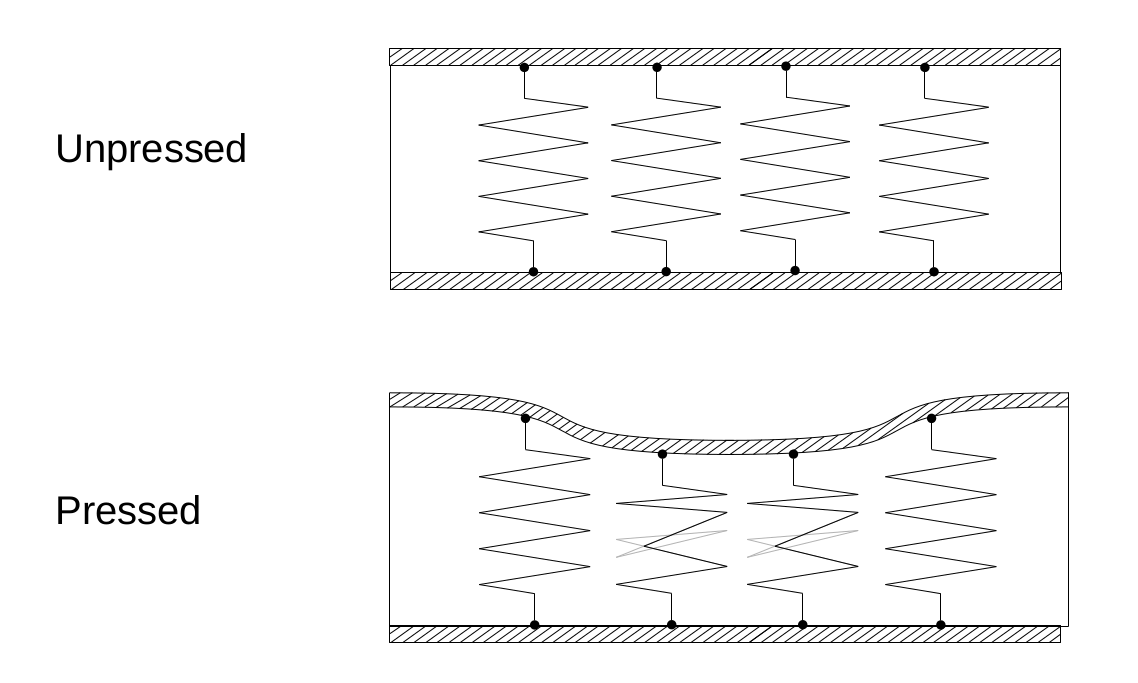
\includegraphics[width=0.9\columnwidth]{figures/resistive_sensor}
  \caption{Conceptual model of a pressure sensor. Compressing the sensor causes
  partial short-circuits which lowers the overall resistance of the
  structure.}~\label{fig:pressure_sensor}
\end{figure}

\subsection{Capacitive Touch / Distance Sensors}
Capacitive sensors are popular sensors in embedded computing due to their low cost
and capabilities of detecting approaching human body parts, which allows the
object to give feedback to the user even before the user is physically touching
the object. The physics behind sensors that meaure self-capacitance is that one
plate of the capacitor is formed by the sensor and the other plate is formed by
nearby grounded objects. The capacitance is a function of area and distance, as
shown by the well-known parallel plate model

\begin{equation}
C = {{\varepsilon A} \over {d}}
\end{equation}

where $C$ is the capacitance, $\varepsilon$ is the permittivity of the material
between the plates (approximately $8.85418 \cdot 10^{-12} ~ \textrm{F/m}$ for
air), $A$ is the overlapping area of the plates and $d$ is the distance between
the plates.

For many use cases of capacitive touch, the permittivity and area do not change
significantly and thus the capacitiance is a measure for the distance between
the sensor and the body part.

There are many different methods to measure
self-capacitance (FIXME: ADD REFERENCE TO RC-DISCHARGE, CVD, RELAXATION
OSCILLATOR, OTHERS?). 

\subsubsection{R-C Charge Method}
A very popular method in the Do It Yourself (DIY) community is the R-C charge
method. In this method, the sensor is connected to a digital input pin of a
microcontroller and a resistor is connected to the sensor and a digital output
pin of the microcontroller. Toggling the output pin causes the capacitive sensor
to charge or discharge. These charge and discharge times depend on the value of
the resistor and the value of the capacitor formed by the sensor plate and the
human body and the microcontroller determines the capacitance by measuring these
charge and discharge times.

The R-C charge method is very simple and low cost as it requires only an
additional resistor and two General Purpose Input Output pins (GPIO pins) of a
microcontroller, which makes it very attractive to the DIY community.  However,
since it is based on measuring charge and discharge times it is also relatively
slow.

An intrinsic feature of capacitive touch sensors is that the
electric field needs to fringe out of the object to be able to sense the human
body and due to this fringing, the electric field is also easily disturbed by
other electric fields or nearby grounded objects such as 110 / 230 V wires or
devices or metal structures. The slow measurement method of the R-C charge
method makes it more difficult to filter out these disturbances, leading to poor
performance of the sensor and poor experiences of capacitive touch for users of
the objects which use this method.

\subsubsection{CVD Method}
Another well-known method for self-capacitance does not rely on R-C charge times
but instead relies on a microcontroller with a multiplexed Analog to Digital
Converter (ADC), the sample-and-hold capacitor ($\textrm{C}_{\textrm{S\&H}}$)
inside this ADC and the ability of the microcontroller to dynamically
reconfigure its analog input pins to digital output pins. This method is called
Capacitive Voltage Division (CVD).

In this method, no external resistor is required and the sensor plate is
directly connected to an analog input pin. The microcontroller starts a
measurement by configuring this pin a digital output and making this output low,
thereby discharging the sensor. Next, the microcontroller connects the internal
ADC to its supply voltage, which charges $\textrm{C}_{\textrm{S\&H}}$ to a fixed
amount of charge which depends only on the capacitance
$\textrm{C}_{\textrm{S\&H}}$ and the supply voltage.

Afther the sensor pin is discharged and $\textrm{C}_{\textrm{S\&H}}$ is
charged, the sensor pin needs to be reconfigured as analog input and the
multiplexer of the ADC needs to be switched to this input. This will
redistribute the charge on $\textrm{C}_{\textrm{S\&H}}$ over both
$\textrm{C}_{\textrm{S\&H}}$ and the capacitance of the sensor. A larger sensor
capacitance will result in a lower voltage on the sensor and the last step of
this method is to measure this voltage using the usual ADC functions.

Since this method does not rely on R-C discharge times but uses the internal and
usually much faster ADC, more filtering can be applied to the signal to remove
disturbance of other nearby objects and electronic devices. This results in a
superior performance and a better user experience.

\subsection{Using Resistive Pressure Sensors as Capacitive Distance Sensors}
The CVD method connects the sensor directly to analog input of a
microcontroller, similar to the resistive sensor setup. The resistive sensor can
now be used to also measure capacitance by connecting the other electrode of the
sensor to a GPIO pin instead of ground. This setup is shown in the side bar

The top diagram shows the setup in resistive sensing mode, which is a standard
resitive divider setup which uses an internal pull resistor as reference
resistor and a digital output pin as ground to complete the circuit.

The bottom diagram shows the same circuit but with the GPIO pins reconfigured
for capacitive sensing. In this setup, the internal pull up resistor is not used
and the to electrode of the pressure sensor is only connected to the analog
input. The bottom electrode is connected to a pin that is configured as digital
input, which effectively means that the sensor is floating. This is exactly the
setup that is needed for the CVD method.

\reversemarginpar
\vspace{-60pt}
\marginnote{
  \hspace{-40pt}
  \fbox{
    \begin{0.9\marginpagewidth}{0.925\marginparwidth}
    \textbf{Circuit for resistive and capacitive sensing}
    {
      \centering
      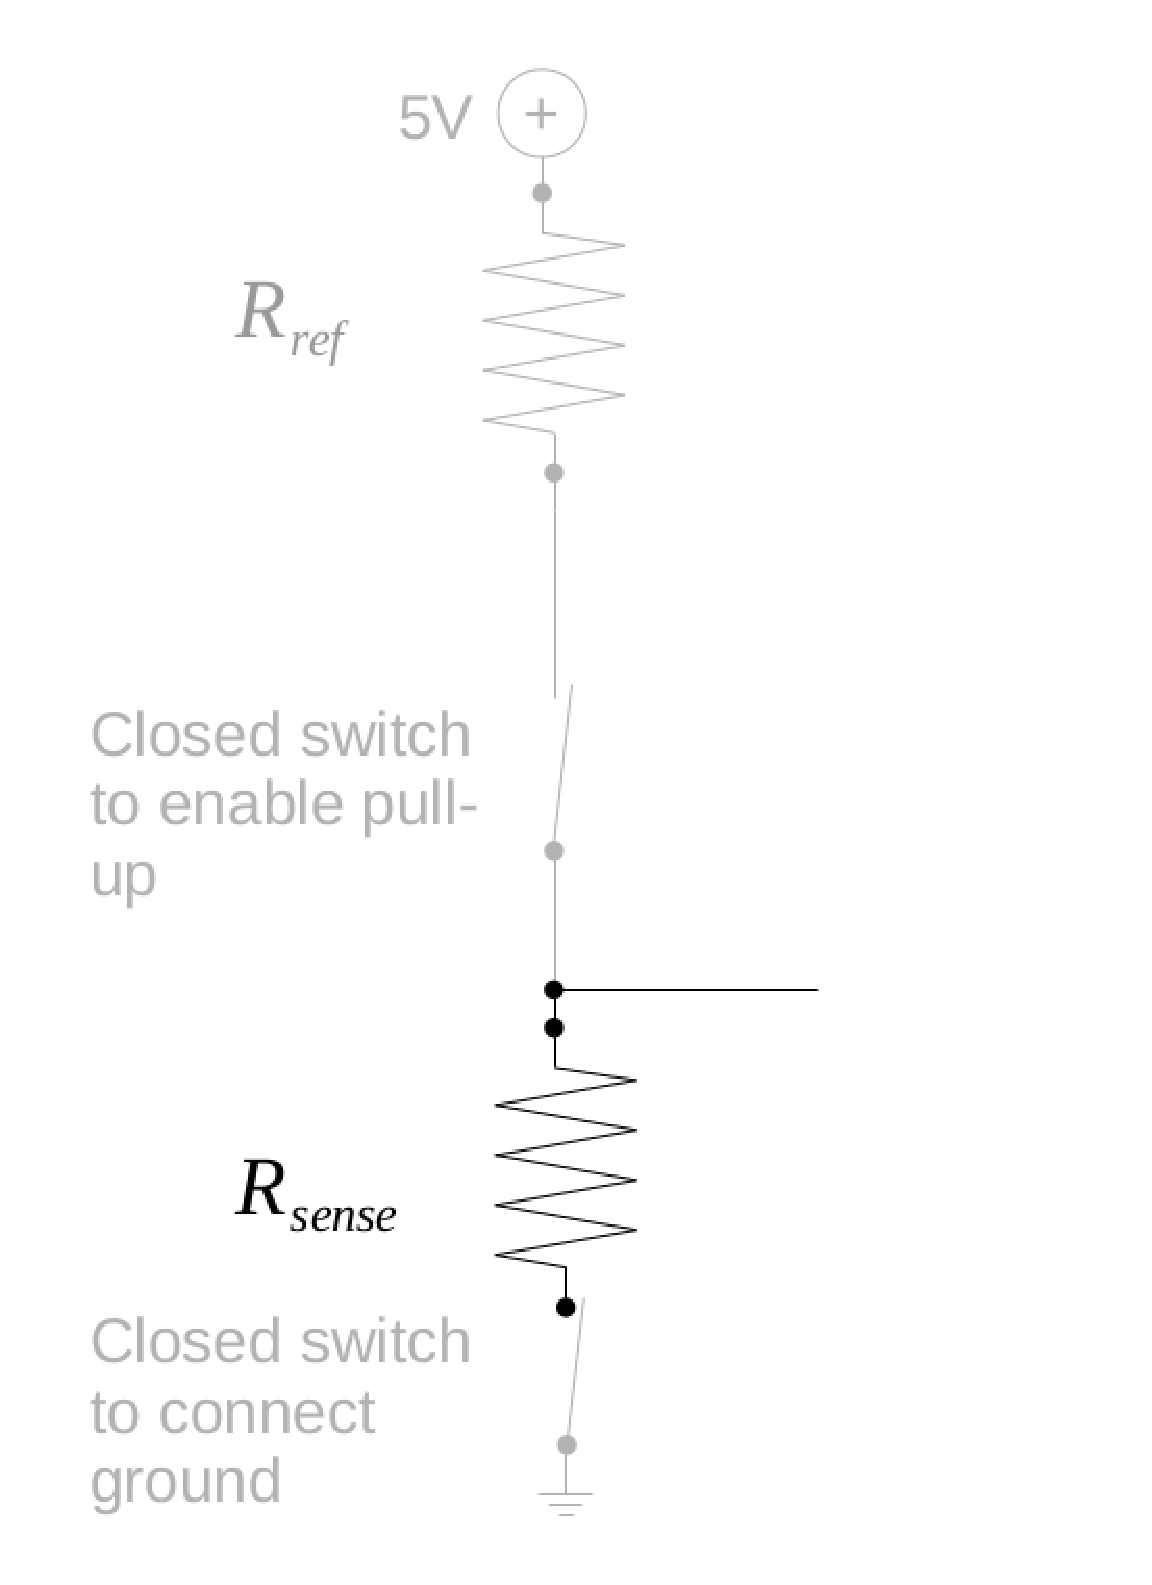
\includegraphics[width=0.85\marginparwidth]{figures/cap_res_setup_res}
      \hline
      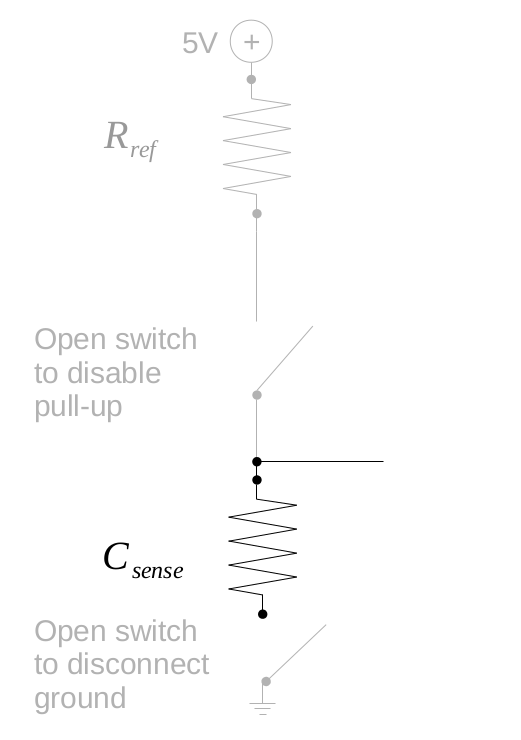
\includegraphics[width=0.85\marginparwidth]{figures/cap_res_setup_cap}
      Resistive pressure sensor used in capacitive and resistive setup. Top: circuit in
      resistive sensing mode. Bottom: circuit in capacitive sensing mode. Grey items are internal to the
      microcontroller.
    }
    \end{0.9\marginpagewidth}
  }
}
\normalmarginpar
\vspace{60pt}

\section{Software Features}
In many cases both resistive pressure sensing and capacitive presence sensing
applications require relative measurements but do not depend on absolute
measurements. In such cases, a state machine which tracks any background
variations on the signal level is a simple and effective method to reduce noise.
In our case, both the resistive sensor signals and the capacitive sensor signals
use the following state machine where each signal has its own instance and
its own parameter settings.

The state machine for each sensor can be in five states:
\begin{itemize}
\item Calibrating
\item Released
\item Released to Pressed
\item Pressed
\item Pressed to Released
\item Released
\end{itemize}
This is shown in Figure \ref{fig:state_machine}.

\begin{figure}[!htbp]
\centering
  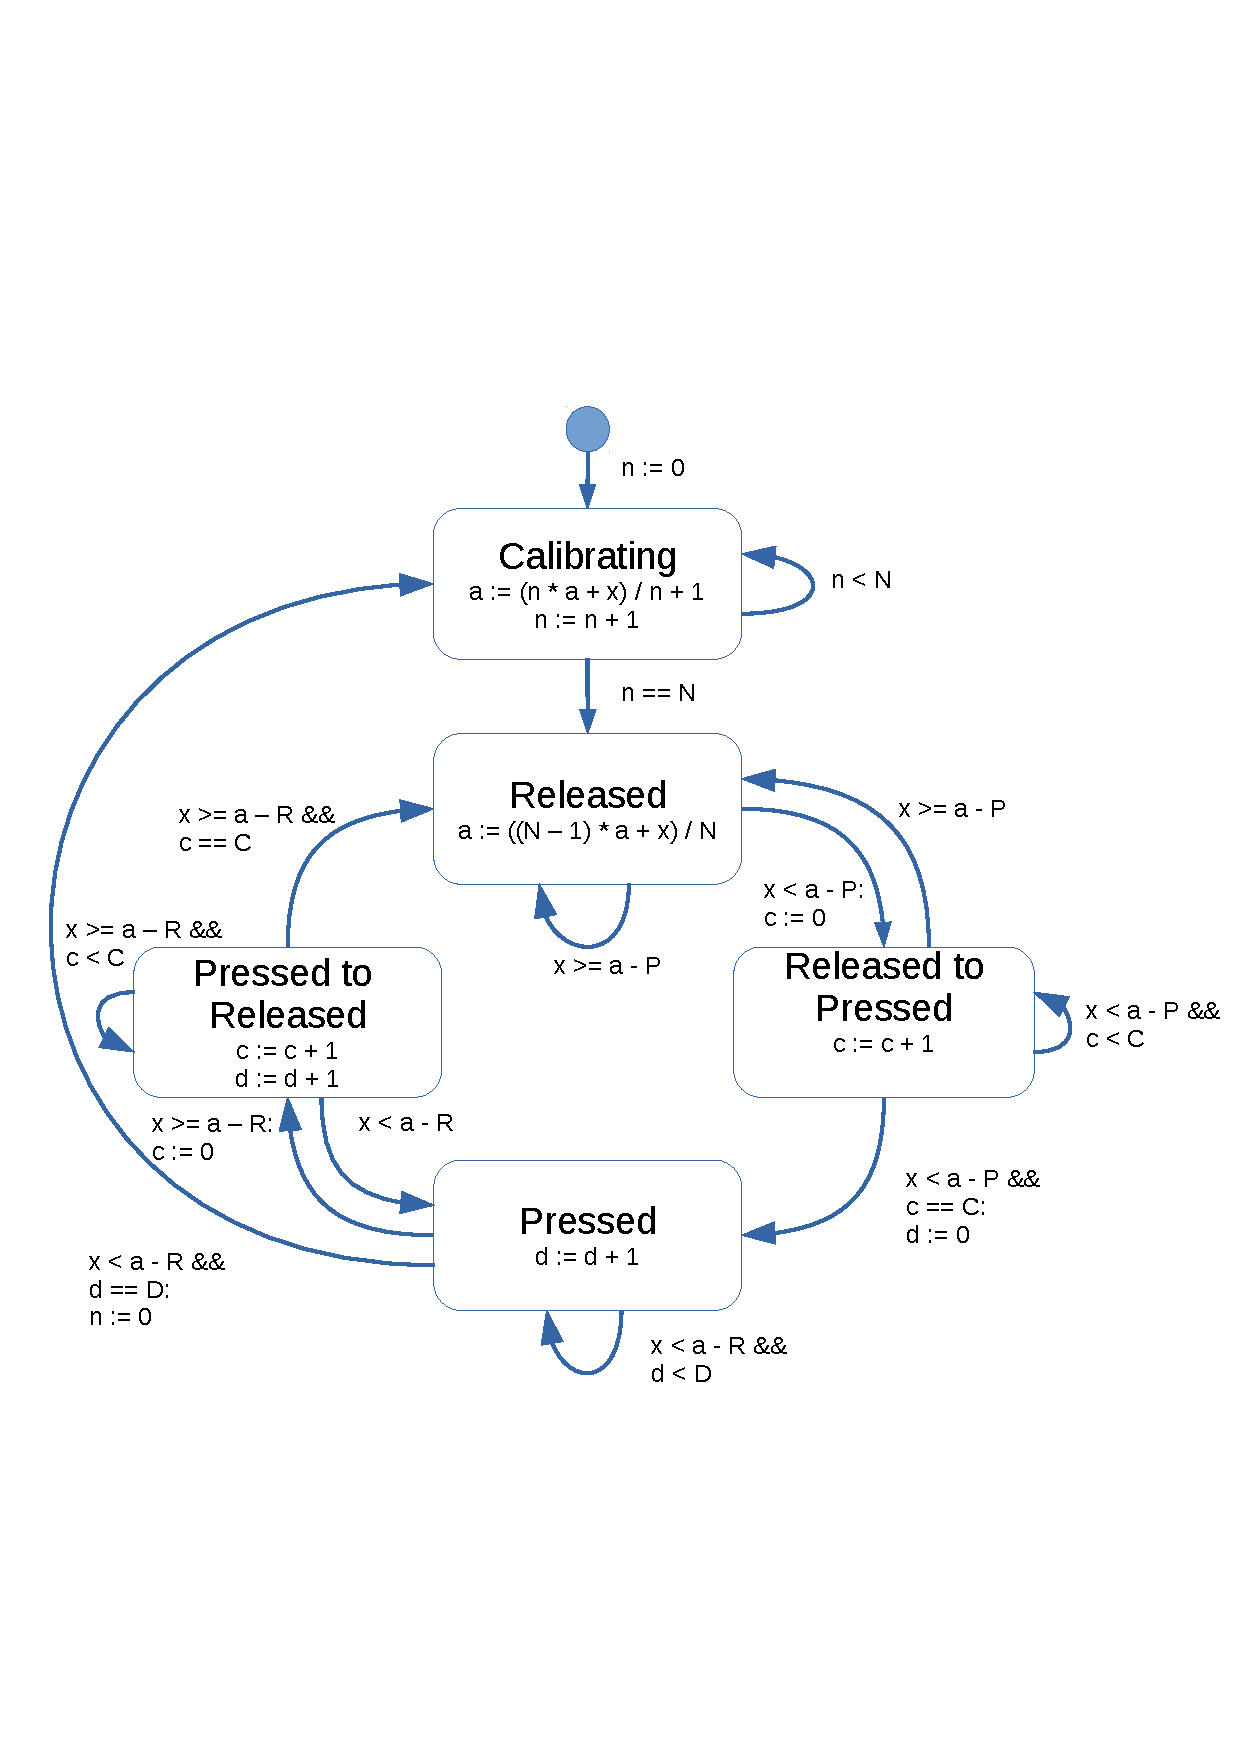
\includegraphics[width=0.9\columnwidth]{figures/state_machine}
  \caption{State machine for resistive and capacitive measurements to track
background variations.}~\label{fig:state_machine}
\end{figure}

In the Calibrating and Released states, the background variations are tracked
using an exponential decaying filter and stored in average $a$. In all other
states the background variations are not tracked. In the Released state, if the
most recent measurement $x$ is more than $P$ counts below average $a$, the state
is changed to Released to Pressed. If in the next measurement $x$ is less
than $P$ counts below the average, the state is changed back to Released. If
however the next $C$ measurements are all more than $P$ counts below this
average, the state is changed to Pressed.

Similarly the state moves from the Pressed state to the Pressed to Released
state and from Pressed to Released to the Released state.

To account for stuck buttons (for example: when the user unintentionally placed
a large conductive object very close to the capacitive touch sensor while the
sensor was in Released state), there is a maximum time that the sensor can be in
the Pressed state. If after this time the sensor is still in the Pressed state,
it is changed to the Calibrating state and the sensor will start recalibrating.

By changing the parameters $N$, $C$, $P$ and $R$ the amount of filtering and
speed of detection can be tuned to the application.

FIXME: ADD REFERENCE TO STATE MACHINE 

\section{Shielding}
In capacitive sensing mode, the bottom electrode of the resistive pressure
sensor is floating. In this mode the pressure sensitive resistive material in
between can be seen effectively as a conductor and thus the whole sensor can be
seen as just a single electrode. The electric field of the sensor will therefore
also fringe all around the sensor, including the bottom side. As the electric
field is also present at the underside of the sensor, the sensor is not only
sensitive for the presence of human body parts above the sensor, but also below.
If the capacitance underneath the sensor is relatively constant, tuning of the
state machine could be sufficient to filter this out and make the sensor only
sensitive to large and / or rapid variations.

However, for some applications such as lose fitting clothing, this might still
not be sufficient. In such cases, the sensor can be made less sensitive by
adding a shield underneath the sensor. Connecting this shield to ground
effectively removes all of the capacitance variation but also reduces the
sensitivity of the sensor. By connecting the sensor itself to the input of a 1 x
opamp and the output of the opamp to the shield, the voltage of the shield is
always very close to the voltage on the sensor itself. As a result, the electric
field underneath the sensor is virtually zero and no sensitivity is lost. Note
that for proper shielding, also the cable to the sensor should be shielded. A
schematic diagram is shown in Figure \ref{fig:shield_circuit}.

FIXME: ADD REFERENCE TO SHIELDING

\begin{figure}[!htbp]
\centering
  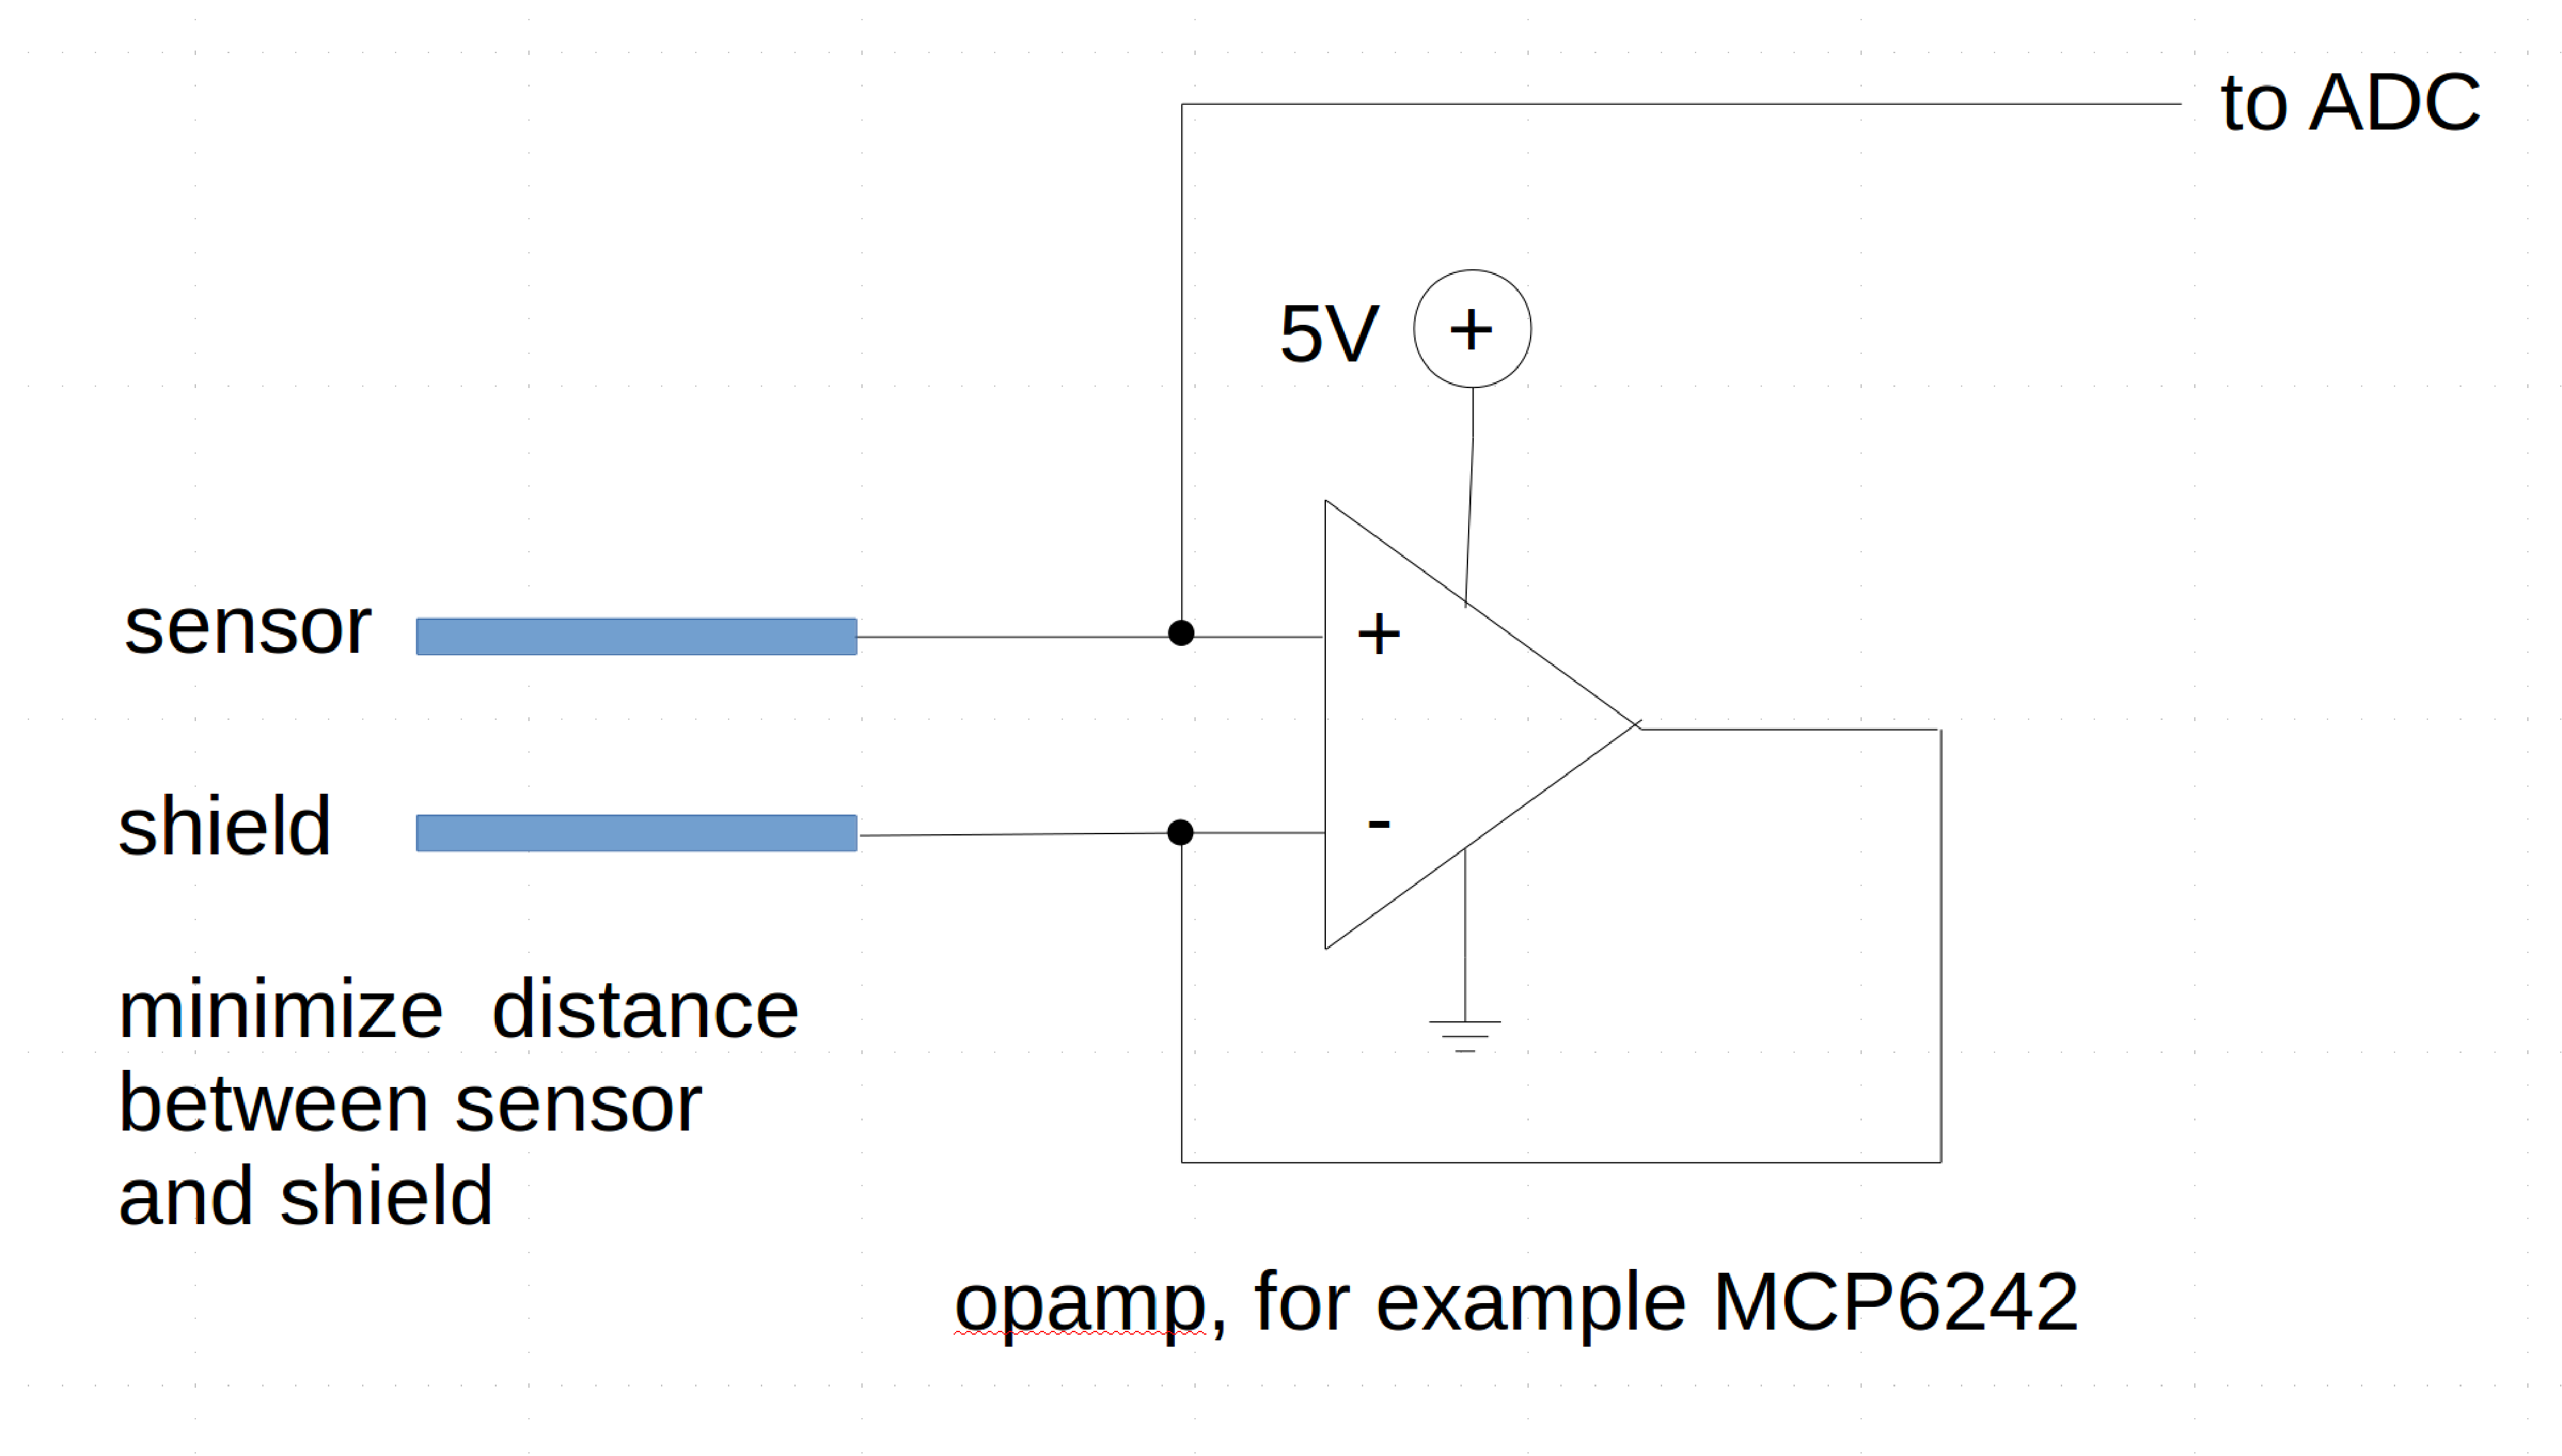
\includegraphics[width=0.9\columnwidth]{figures/shield_circuit}
  \caption{Circuit to shield underside of capacitive
sensor.}~\label{fig:shield_circuit}
\end{figure}

\section{Mechanical Features}
An overview of the stackup of the total sensor is shown in Figure
\ref{fig:stackup}. In this figure, the electrode and shield material can be
conductive textile, the insulating material can be any non-compressable
insulating material (for example cotton) and the pressure sensitive material can
be Velostat or ESD foam.

\begin{figure}[!htbp]
\centering
  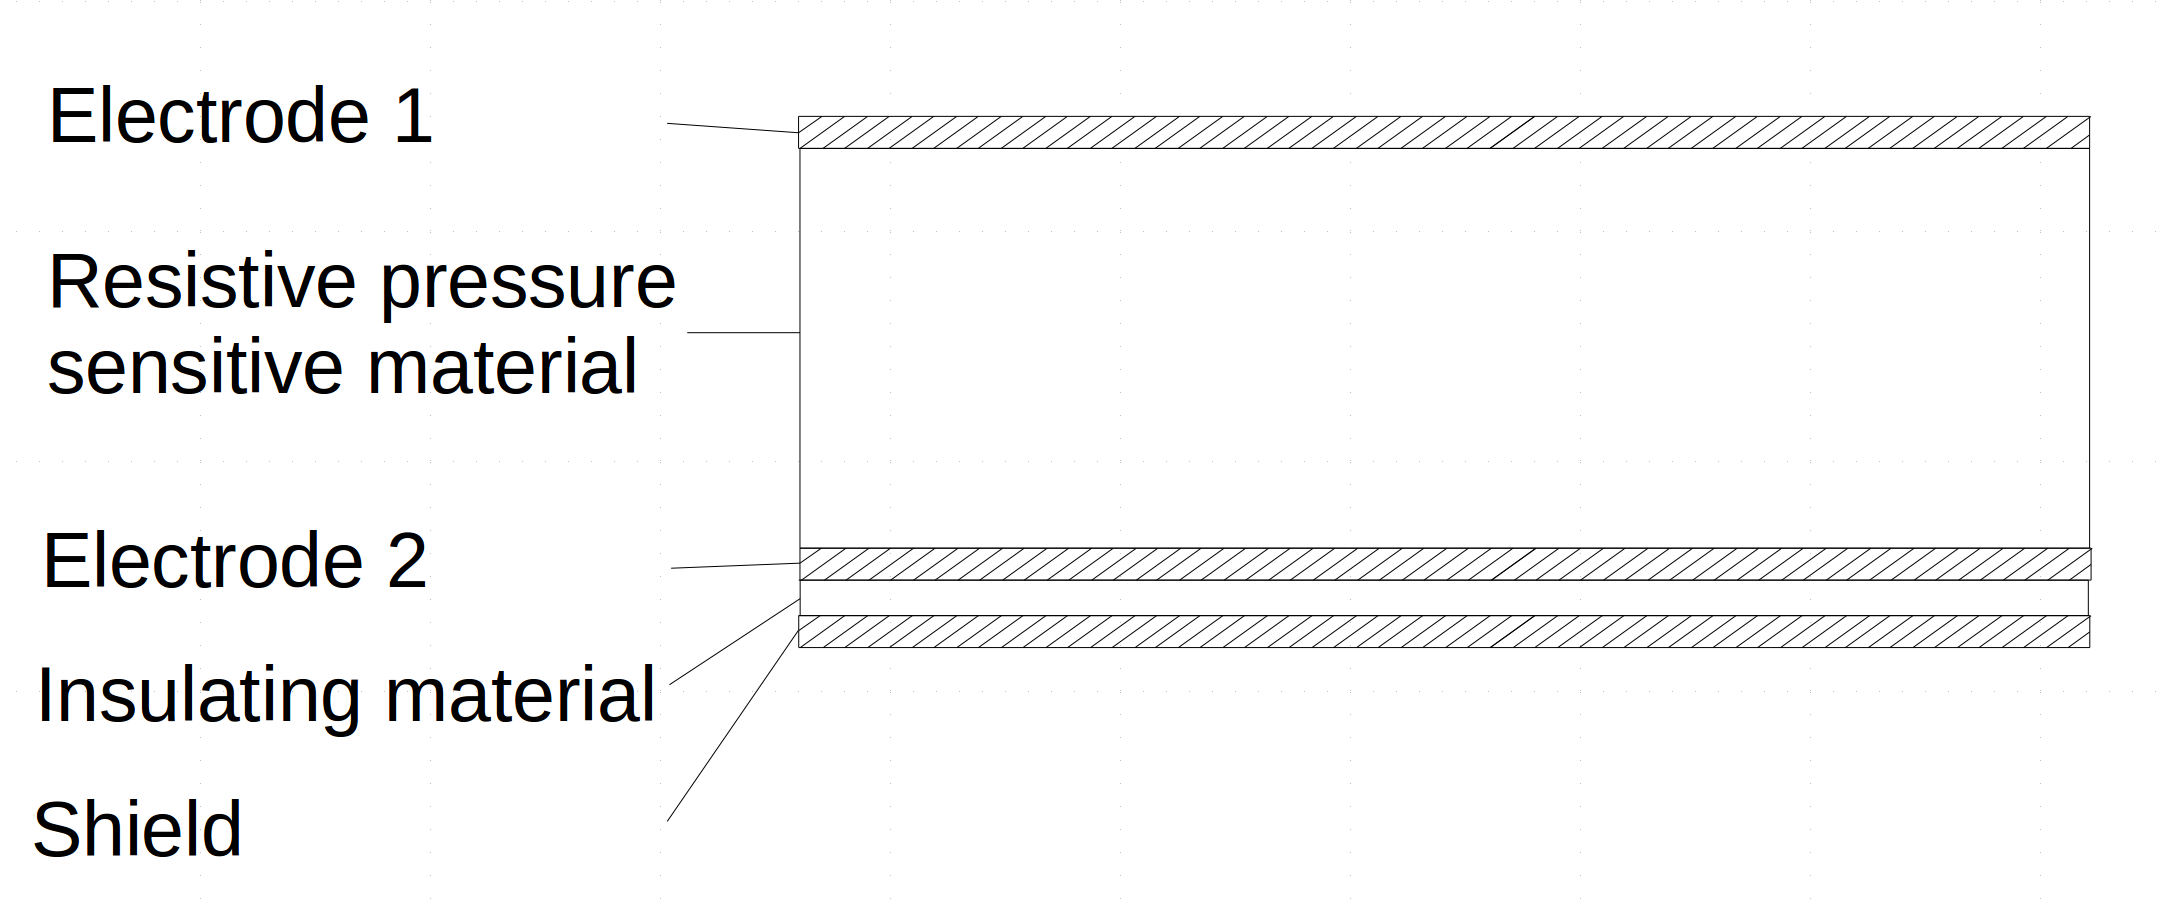
\includegraphics[width=0.9\columnwidth]{figures/stackup}
  \caption{Stackup for pressure and presence sensor with
shield}~\label{fig:stackup}
\end{figure}


\section{Conclusion}
In this paper we have described the combination of capacitive distance sensing
using the CVD method for presence sensing with resistive sensing for pressure
sensing. The robustness of the CVD method as well as the required circuit and
microcontroller features make it ideal to combine with existing resistive
pressure sensing applications to enhance the user experience by not only sensing
how hard a user presses on a button but already giving feedback to the user when
he / she is approaching the button.
% BALANCE COLUMNS
\balance{} 
% REFERENCES FORMAT
% References must be the same font size as other body text.
\bibliographystyle{SIGCHI-Reference-Format}
\bibliography{sample}

\end{document}

%%% Local Variables:
%%% mode: latex
%%% TeX-master: t
%%% End:
